%%%%%%%%%%%%%%%%%%%%%%%%%%%%%%%%%%%%%%%%%%%%%%%%%%%
% glaubergribov.tex
% Author: Gunter Folger, Vladimir Grichine
%%%%%%%%%%%%%%%%%%%%%%%%%%%%%%%%%%%%%%%%%%%%%%%%%%%
\paragraph{Glauber-Gribov extension}
The simplified Glauber model cross sections assume Gaussian-distributed,
point-like nucleons and are given by~\cite{hadbib:ggepjc,hadbib:ggnimb}:
\[
\sigma^{hA}_{tot}=2\pi R^2\ln\left[1+\frac{A\sigma^{hN}_{tot}}{2\pi R^2}\right],\quad
\sigma^{hA}_{in} = \pi R^2\ln\left[1+\frac{A\sigma^{hN}_{tot}}{\pi R^2}\right],
\]
\[
\quad \sigma^{hA}_{el}=\sigma^{hA}_{tot}-\sigma^{hA}_{in}.
\]
Here $\sigma^{hA}_{tot}$, $\sigma^{hA}_{in}$, and $\sigma^{hA}_{el}$ are the
total, inelastic and elastic cross sections, respectively. 

The model is reduced to the selection of $\sigma^{hN}_{tot}$ and $R(A)$
values.  The latest edition of PDG \cite{hadbib:PDG} and \Gfour{} parameterizations
were used for $\sigma^{hN}_{tot}$, including the total cross sections of $p$,
$\bar{p}$, $n$, $\pi^{\pm}$, $K^{\pm}$ and $\Sigma^{-}$ on protons and neutrons
% (http://pdg.lbl.gov/2006/reviews/hadronicrpp.pdf).  
For known cross sections on protons and neutrons,
$A\sigma^{hN}_{tot}=N_{p}\sigma^{hp}_{tot}+N_{n}\sigma^{hn}_{tot}$, where $N_{p}$
and $N_{n}$ are the number of protons and neutrons in the nucleus.
The nuclear radius (the RMS radius of the nucleon Gaussian distribution), 
is parametrized as $R(A) = r_{o}A^{\frac{1}{3}}f(A)$, 
$r_{o} \sim 1.1 \ fm$, with $f(A) < 1$ for $A > 21$, and $f(A) > 1$ for the  
case $3 < A < 21$. 
Figures \ref{nCtotinprodGG} and \ref{pCinprodBGG} show the prediction of the
Barashenkov and Glauber-Gribov model for total, inelastic and production cross
sections of neutrons and protons on a carbon target.  The production cross
section is defined to be the difference between the inelastic and charge 
exchange cross sections.  

\begin{figure}
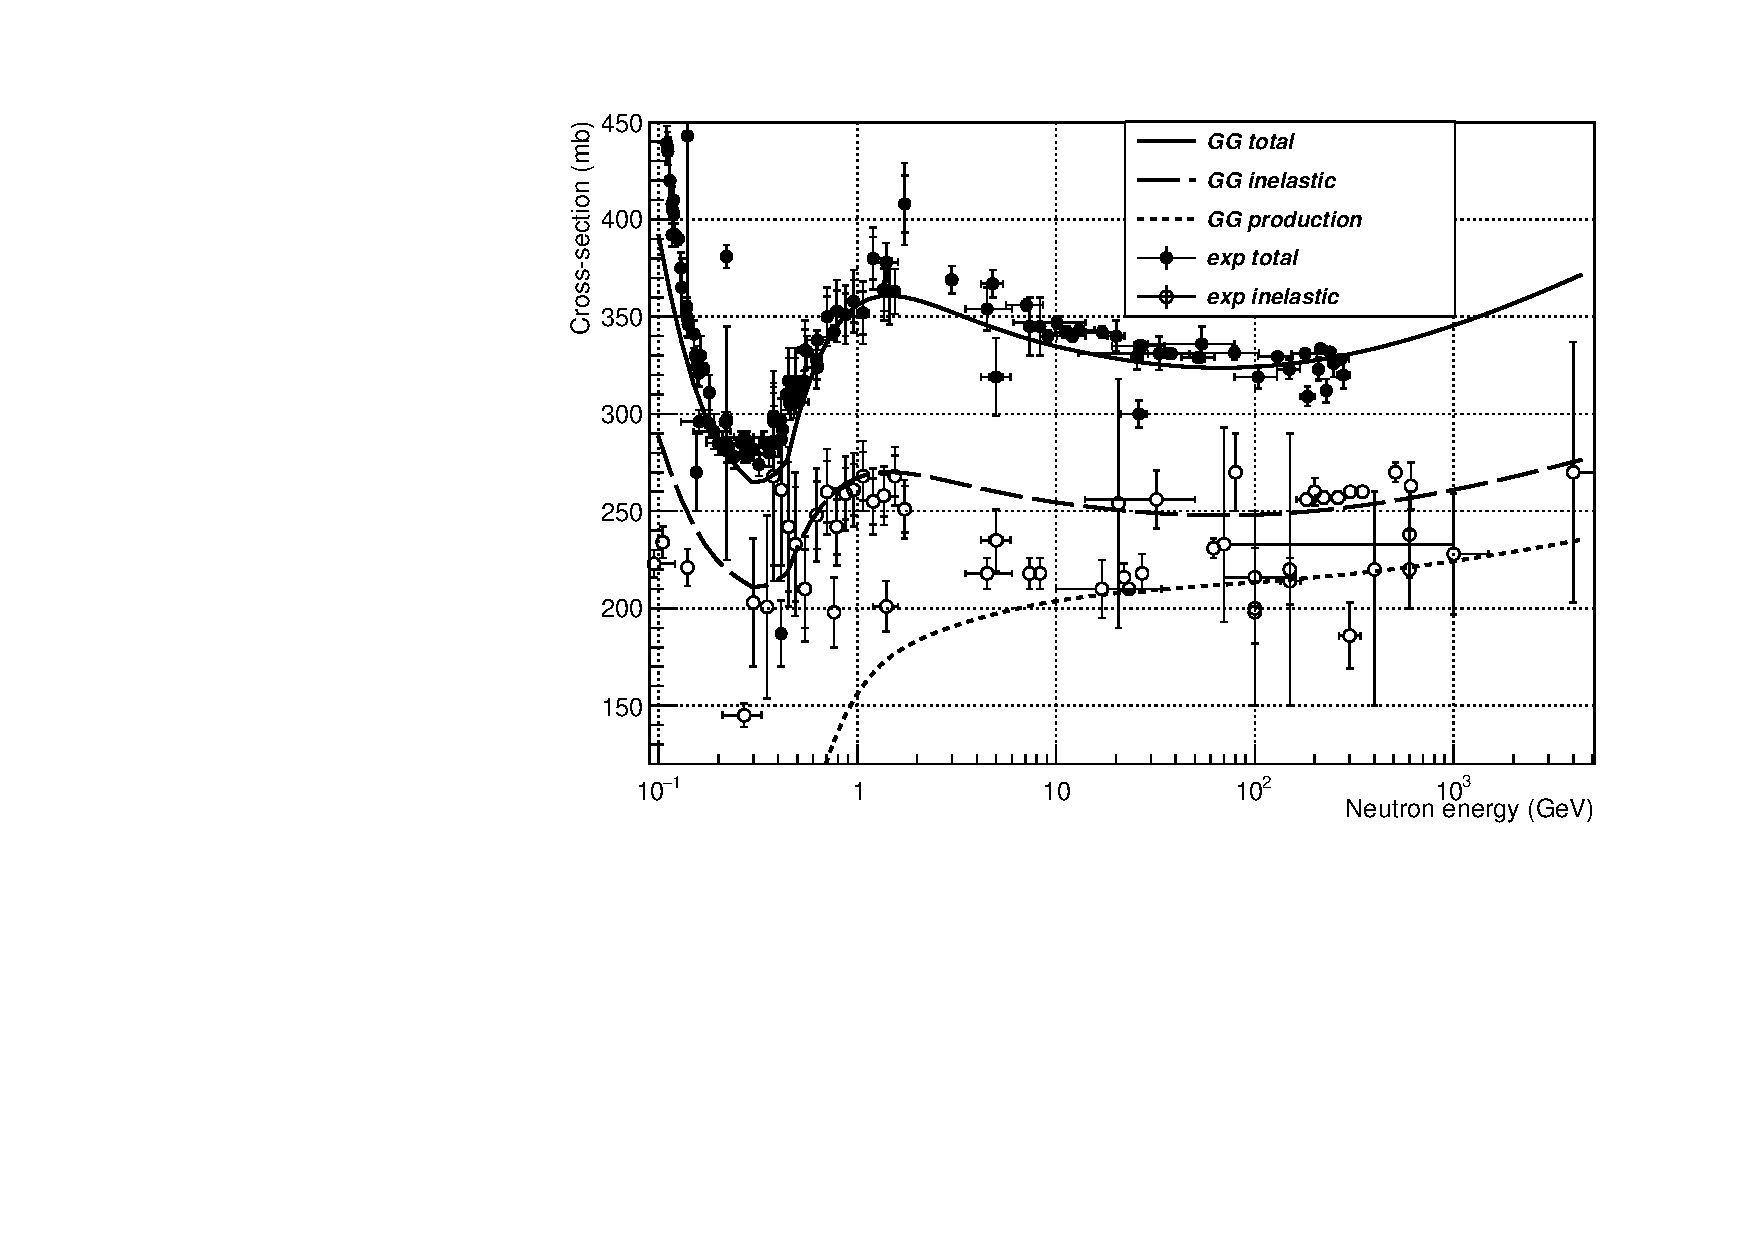
\includegraphics[width=0.5\textwidth]{figures/nCtotinprodGG.pdf}
% \centering \includegraphics[height=3.3in,width=3.6in]{figures/nCtotinprodGG.eps}
\caption{ Total, inelastic and production cross-sections of neutrons on a carbon 
target in the energy range $10^{-2}-10^3$~GeV. Experimental data (open and solid
points) from \cite{hadbib:ihepbase,hadbib:dubnabase}, lines correspond to the 
Glauber-Gribov model.}
\label{nCtotinprodGG}
\end{figure}

\begin{figure}
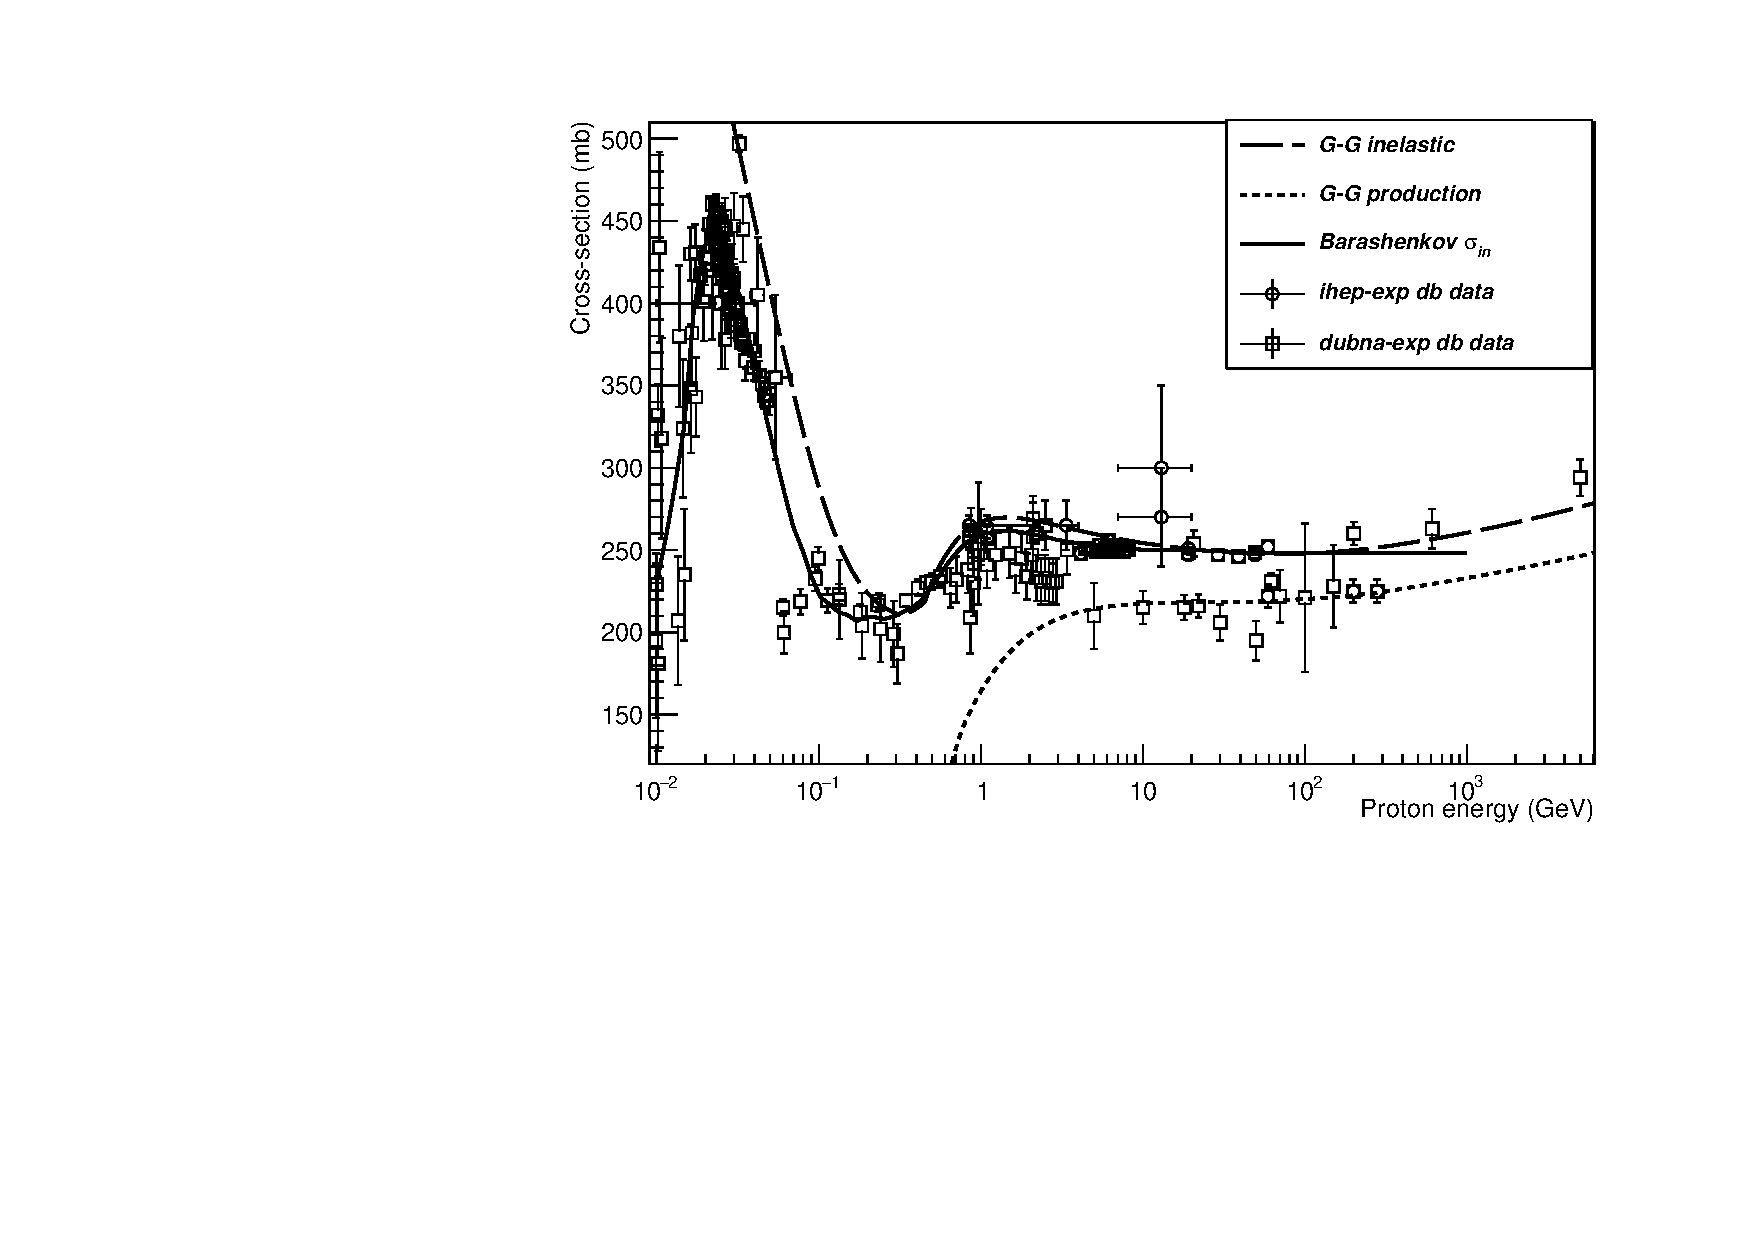
\includegraphics[width=0.5\textwidth]{figures/pCinprodBGG.pdf}
% \centering \includegraphics[height=3.3in,width=3.6in]{figures/pCinprodBGG.eps}
\caption{ Inelastic and production cross-sections of protons on a carbon 
target in the energy range $10^{-2}-10^3$~GeV. Experimental data (open points
and squares) are from \cite{hadbib:ihepbase,hadbib:dubnabase}. The solid and 
dashed lines correspond to the Barashenkov and Glauber-Gribov inelastic models,
respectively.  The dotted line shows the Glauber-Gribov production model.}
\label{pCinprodBGG}
\end{figure}



